% Author: Izaak Neutelings (July 2017)
\documentclass[border=3pt,tikz]{standalone}
\usepackage{amsmath} % for \text
\usepackage{tikz}
\tikzset{>=latex} % for LaTeX arrow head
\usetikzlibrary{decorations.markings} % for arrow
\usetikzlibrary{decorations.pathmorphing} % for snake
\usetikzlibrary{shadows.blur}

% CUSTOM VERTICAL SHADING
%https://tex.stackexchange.com/questions/191735/is-it-possible-to-define-the-position-of-top-bottom-and-middle-color-in-fill
\makeatletter
\tikzset{vertical custom shading/.code={%
  \pgfmathsetmacro\tikz@vcs@middle{#1}
  \pgfmathsetmacro\tikz@vcs@bottom{\tikz@vcs@middle/2}
  \pgfmathsetmacro\tikz@vcs@top{(100-\tikz@vcs@middle)/2+\tikz@vcs@middle}
  \pgfdeclareverticalshading[tikz@axis@top,tikz@axis@middle,tikz@axis@bottom]{newaxis}{100bp}{%
    color(0bp)=(tikz@axis@bottom);
    color(\tikz@vcs@bottom bp)=(tikz@axis@bottom);
    color(\tikz@vcs@middle bp)=(tikz@axis@middle);
    color(\tikz@vcs@top bp)=(tikz@axis@top);
    color(100bp)=(tikz@axis@top)}
    \pgfkeysalso{/tikz/shading=newaxis}
  }
}
\makeatother

% PARTICLE STYLES
\colorlet{myblue}{blue!40!black}
\colorlet{trackcol}{orange!50!red!50!black}
\colorlet{ECALcol}{green!30!black}
\colorlet{HCALcol}{blue!50!black}
\colorlet{photoncol}{orange!60!yellow!90!black}
\colorlet{hadroncol}{red!60!black}
\colorlet{taucol}{blue!60!black}
\colorlet{rhocol}{green!60!black}
\colorlet{a1col}{blue!40!black}
\tikzset{
  ->-/.style={decoration={markings,mark=at position .7 with {\arrow{>}}},
                          postaction={decorate}},
  photon/.style={decorate,decoration={snake,segment length=5,amplitude=1.1}},
  charged/.style={->-,thick,hadroncol!20!black}, %,line cap=round
  neutral/.style={->-,densely dashed,thick},
  neutrino/.style={->-,dotted,thick},
  cone/.pic={
    \shadedraw[#1!90!black,top color=white,bottom color=#1!50,shading angle=50,vertical custom shading=10]
               (-0.4,0.99) -- (0,0) -- (0.4,0.99);
    \shadedraw[#1!90!black,top color=white,bottom color=#1!20,shading angle=90]
               (0,1) ellipse (0.4 and 0.12);},
  pics/cone/.default=hadroncol!20!black,
}

% SUBDETECTOR
\def\subdetedge#1{ ({(\R+#1)*sin(\hca)},{#1+(\R+#1)*(cos(\hca)-1)}) } % edge
\def\subdetectors{
  \def\hclmax{(\R+\HCAL)*sin(\hca)} % max
  \foreach \r in {\tracker,\ECAL,\HCAL}{
    \coordinate (Edge) at ({(\R+\r)*sin(\hca)},{\r+(\R+\r)*(cos(\hca)-1)});
    \draw[thick] (Edge) arc (90-\hca:90+\hca:\R+\r);
  }
  \node[left=0,above left] at ({1.1*\hclmax},0.2*\tracker) {tracker};
  \node[left=0,above left] at ({1.1*\hclmax},\tracker) {ECAL};
  \node[left=0,above left] at ({1.1*\hclmax},\ECAL) {HCAL};
}
\def\subdetectorscol{ % colored
  \def\rmin{-0.4} % max
  \def\hclmax{(\R+\HCAL)*sin(\hca)} % max
  \foreach \r/\col in {\HCAL/HCALcol,\ECAL/ECALcol,\tracker/trackcol}{
    \coordinate (Edge1) at ({-(\R+\rmin)*sin(\hca)},{\rmin+(\R+\rmin)*(cos(\hca)-1)});
    \coordinate (Edge2) at ({(\R+\r)*sin(\hca)},{\r+(\R+\r)*(cos(\hca)-1)});
    \fill[top color=\col!10,bottom color=\col!4,shading angle=12]
      (Edge1) --++ ({2*(\R+\rmin)*sin(\hca)},0) -- (Edge2)
      arc (90-\hca:90+\hca:\R+\r) -- cycle;
    \draw[thick,\col] (Edge2) arc (90-\hca:90+\hca:\R+\r);
  }
  \node[left=0,above left,trackcol] at ({1.1*\hclmax},0.2*\tracker) {tracker};
  \node[left=0,above left,ECALcol] at ({1.1*\hclmax},\tracker) {ECAL};
  \node[left=0,above left,HCALcol] at ({1.1*\hclmax},\ECAL) {HCAL};
}


\begin{document}
\large


% TAU DECAY MODES 0, 1, 10, 11
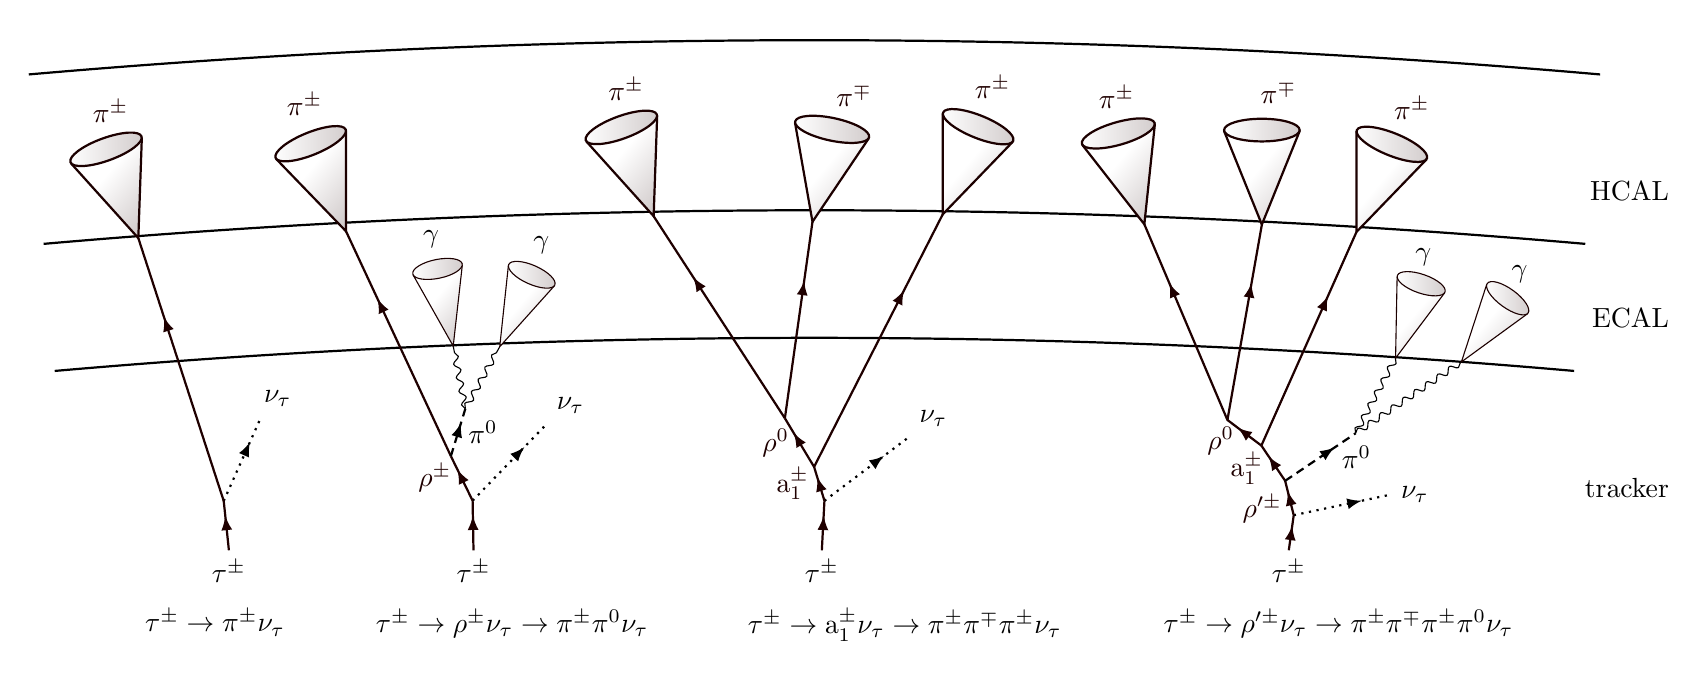
\begin{tikzpicture}[scale=0.9]
  \def\R{120}            % inner radius
  \def\hca{5}            % half central angle
  \def\hcl{\R*sin(\hca)} % half chord length c = 2Rsin(theta/2)
  \def\tracker{3}        % tracker
  \def\ECAL{4.8}         % ECAL
  \def\HCAL{7.2}         % HCAL
  
  % SUBDETECTORS
  \subdetectors
  
  % DM 0
  \begin{scope}[shift={({-0.79*\hcl},0)},rotate=6]
    \node[below] at (0,0) {$\tau^\pm$};
    \node[left=5,below=18] at (0,0) {$\tau^\pm\to\pi^\pm\nu_\tau$};
    \draw[charged] % tau
      (0,0) -- (0,0.7) coordinate (tau);
    \draw[neutrino,rotate=-30] % neutrinos
      (tau) --+ (0,1.3) node[right=6pt,above] {$\nu_\tau$};
    \draw[charged,rotate=12] % pion
      (tau) --+ (0,3.9) node[left=10,above=38] {$\pi^\pm$}
      pic[rotate=20,scale=1.2] {cone};
  \end{scope}
  
  % DM 1
  \begin{scope}[shift={({-0.46*\hcl},0)},rotate=1]
    \node[below] at (0,0) {$\tau^\pm$};
    \node[right=14,below=18] at (0,0) {$\tau^\pm\to\rho^\pm\nu_\tau\to\pi^\pm\pi^0\nu_\tau$};
    \draw[charged] % tau
      (0,0) -- (0,0.7) coordinate (tau);
    \draw[neutrino] % neutrinos
      (tau) --+ (45:1.5) node[above right] {$\nu_\tau$};
    \draw[charged] % rho
      (tau) --+ (115:0.7) coordinate (rho) node[midway,left] {$\rho^\pm$};
    \draw[charged] % pion
      (rho) --+ (114:3.5) node[left=15,above=38] {$\pi^\pm$}
      pic[rotate=22,scale=1.2] {cone};
    \draw[neutral] % pion0
      (rho) --+ (72:0.7) coordinate (pion0) node[midway,right] {$\pi^0$};
    \draw[photon] % photon 1
      (pion0) --+ (100:0.9) node[left=8,above=32] {$\gamma$}
      pic[rotate=11.5,xscale=0.8] {cone};
    \draw[photon] % photon 2
      (pion0) --+ (60:1.0) node[right=15,above=30] {$\gamma$}
      pic[rotate=-24,xscale=0.8] {cone};
  \end{scope}
  
  % DM 10
  \begin{scope}[shift={({0.01*\hcl},0)},rotate=-3]
    \node[below] (0,0) {$\tau^\pm$};
    \node[right=30,below=18] at (0,0) {$\tau^\pm\to\text{a}_1^\pm\nu_\tau\to\pi^\pm\pi^\mp\pi^\pm\nu_\tau$};
    \draw[charged] % tau
      (0,0) -- (0,0.7) coordinate (tau);
    \draw[neutrino] % neutrinos
      (tau) --+ (40:1.5) node[above right] {$\nu_\tau$};
    \draw[charged] % a1
      (tau) --+ (110:0.5) coordinate (a1) node[midway,left] {$\text{a}_1^\pm$};
    \draw[charged] % rho
      (a1) --+ (124:0.8) coordinate (rho) node[midway,left] {$\rho^0$};
    \draw[charged] % pion 1
      (rho) --+ (126:3.4) node[left=10,above=38] {$\pi^\pm$}
      pic[rotate=20,scale=1.2] {cone};
    \draw[charged] % pion 2
      (rho) --+ (85:2.8) node[right=15,above=38] {$\pi^\mp$}
      pic[rotate=-12,scale=1.2] {cone};
    \draw[charged] % pion 3
      (a1) --+ (66:4.0) node[right=18,above=38] {$\pi^\pm$}
      pic[rotate=-22,scale=1.2] {cone};
  \end{scope}
  
  % DM 11
  \begin{scope}[shift={({0.64*\hcl},0)},rotate=-6]
    \node[below] (0,0) {$\tau^\pm$};
    \node[right=18,below=18] at (0,0) {$\tau^\pm\to\rho'^\pm\nu_\tau\to\pi^\pm\pi^\mp\pi^\pm\pi^0\nu_\tau$};
    \draw[charged] % tau
      (0,0) -- (88:0.5) coordinate (tau);
    \draw[neutrino] % neutrinos
      (tau) --+ (18:1.4) node[right] {$\nu_\tau$};
    \draw[charged] % rho'
      (tau) --+ (110:0.5) coordinate (rho') node[midway,below=4,left=-1] {$\rho'^\pm$};
    \draw[charged] % a1
      (rho') --+ (130:0.6) coordinate (a1) node[midway,below=2,left] {$\text{a}_1^\pm$};
    \draw[charged] % rho
      (a1) --+ (149:0.6) coordinate (rho) node[midway,below=3,left] {$\rho^0$};
    \draw[charged,line cap=round] % pion 1
      (rho) --+ (119:3.0) node[left=10,above=38] {$\pi^\pm$}
      pic[rotate=16,scale=1.2] {cone};
    \draw[charged,line cap=round] % pion 2
      (rho) --+ (86:2.8) node[right=6,above=40] {$\pi^\mp$}
      pic[rotate=0,scale=1.2] {cone};
    \draw[charged] % pion 3
      (a1) --+ (72:3.3) node[right=20,above=37] {$\pi^\pm$}
      pic[rotate=-22,scale=1.2] {cone};
    \draw[neutral] % pion0
      (rho') --+ (40:1.2) coordinate (pion0) node[midway,above=0,right=4] {$\pi^0$};
    \draw[photon] % photon 1
      (pion0) --+ (68:1.2) node[right=10,above=30] {$\gamma$}
      pic[rotate=-19,xscale=0.8] {cone};
    \draw[photon] % photon 2
      (pion0) --+ (40:1.8) node[right=21,above=25] {$\gamma$}
      pic[rotate=-36,xscale=0.8] {cone};
  
  \end{scope}
  
\end{tikzpicture}


% TAU DECAY MODES 0, 1, 10, 11 - colored
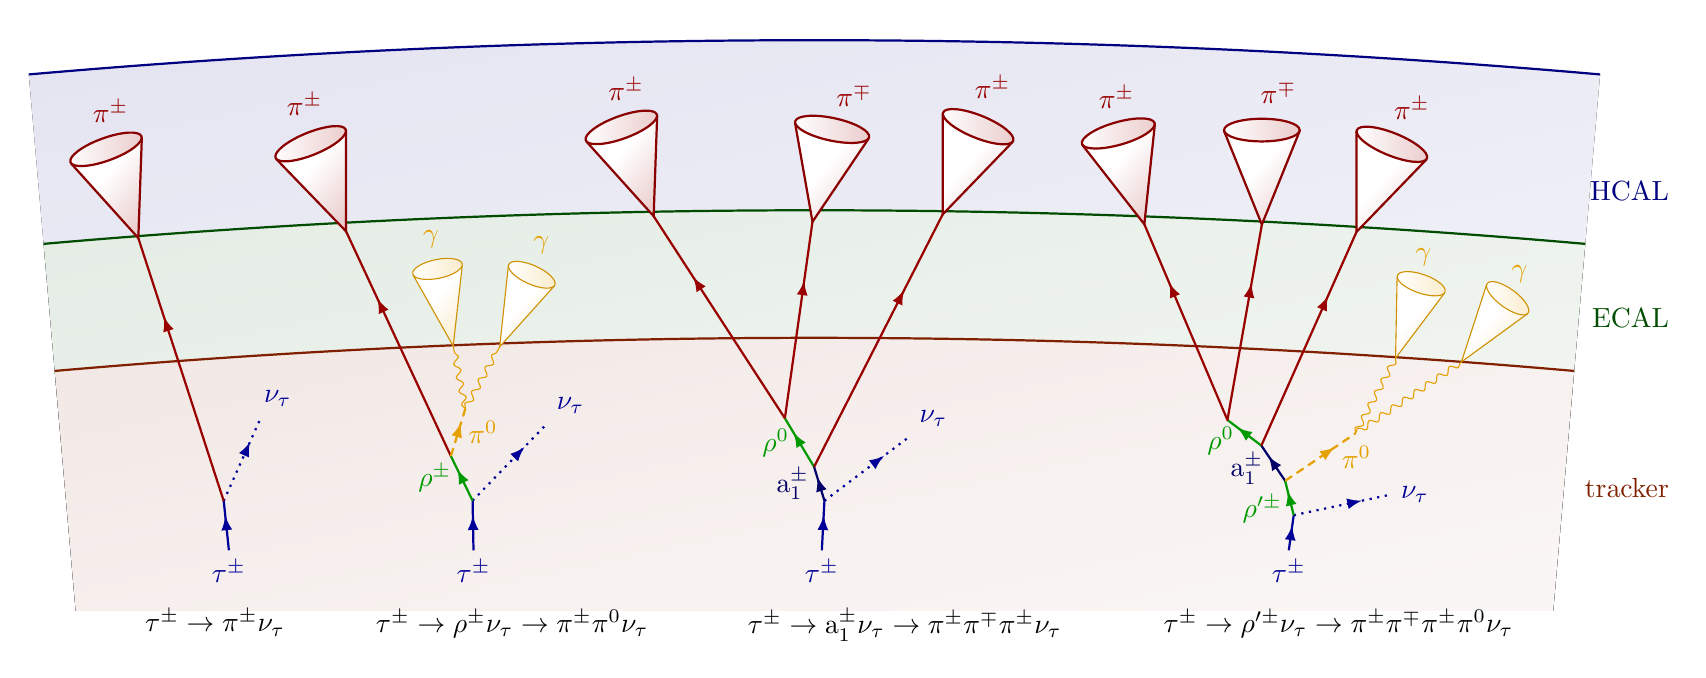
\begin{tikzpicture}[scale=0.9]
  \def\R{120}            % inner radius
  \def\hca{5}            % half central angle
  \def\hcl{\R*sin(\hca)} % half chord length c = 2Rsin(theta/2)
  \def\tracker{3}        % tracker
  \def\ECAL{4.8}         % ECAL
  \def\HCAL{7.2}         % HCAL
  
  % SUBDETECTORS
  \subdetectorscol
  
  % DM 0
  \begin{scope}[shift={({-0.79*\hcl},0)},rotate=6]
    \node[below,taucol] at (0,0) {$\tau^\pm$};
    \node[left=5,below=18] at (0,0) {$\tau^\pm\to\pi^\pm\nu_\tau$};
    \draw[charged,taucol] % tau
      (0,0) -- (0,0.7) coordinate (tau);
    \draw[neutrino,rotate=-30,taucol] % neutrinos
      (tau) --+ (0,1.3) node[right=6pt,above] {$\nu_\tau$};
    \draw[charged,hadroncol,rotate=12] % pion
      (tau) --+ (0,3.9) node[left=10,above=38] {$\pi^\pm$}
      pic[rotate=20,scale=1.2] {cone=hadroncol};
  \end{scope}
  
  % DM 1
  \begin{scope}[shift={({-0.46*\hcl},0)},rotate=1]
    \node[below,taucol] at (0,0) {$\tau^\pm$};
    \node[right=14,below=18] at (0,0) {$\tau^\pm\to\rho^\pm\nu_\tau\to\pi^\pm\pi^0\nu_\tau$};
    \draw[charged,taucol] % tau
      (0,0) -- (0,0.7) coordinate (tau);
    \draw[neutrino,taucol] % neutrinos
      (tau) --+ (45:1.5) node[above right] {$\nu_\tau$};
    \draw[charged,rhocol] % rho
      (tau) --+ (115:0.7) coordinate (rho) node[midway,left] {$\rho^\pm$};
    \draw[charged,hadroncol] % pion
      (rho) --+ (114:3.5) node[left=15,above=38] {$\pi^\pm$}
      pic[rotate=22,scale=1.2] {cone=hadroncol};
    \draw[neutral,photoncol] % pion0
      (rho) --+ (72:0.7) coordinate (pion0) node[midway,right] {$\pi^0$};
    \draw[photon,photoncol] % photon 1
      (pion0) --+ (100:0.9) node[left=8,above=32] {$\gamma$}
      pic[rotate=11.5,xscale=0.8] {cone=photoncol};
    \draw[photon,photoncol] % photon 2
      (pion0) --+ (60:1.0) node[right=15,above=30] {$\gamma$}
      pic[rotate=-24,xscale=0.8] {cone=photoncol};
  \end{scope}
  
  % DM 10
  \begin{scope}[shift={({0.01*\hcl},0)},rotate=-3]
    \node[below,taucol] (0,0) {$\tau^\pm$};
    \node[right=30,below=18] at (0,0) {$\tau^\pm\to\text{a}_1^\pm\nu_\tau\to\pi^\pm\pi^\mp\pi^\pm\nu_\tau$};
    \draw[charged,taucol] % tau
      (0,0) -- (0,0.7) coordinate (tau);
    \draw[neutrino,taucol] % neutrinos
      (tau) --+ (40:1.5) node[above right] {$\nu_\tau$};
    \draw[charged,a1col] % a1
      (tau) --+ (110:0.5) coordinate (a1) node[midway,left] {$\text{a}_1^\pm$};
    \draw[charged,rhocol] % rho
      (a1) --+ (124:0.8) coordinate (rho) node[midway,left] {$\rho^0$};
    \draw[charged,hadroncol] % pion 1
      (rho) --+ (126:3.4) node[left=10,above=38] {$\pi^\pm$}
      pic[rotate=20,scale=1.2] {cone=hadroncol};
    \draw[charged,hadroncol] % pion 2
      (rho) --+ (85:2.8) node[right=15,above=38] {$\pi^\mp$}
      pic[rotate=-12,scale=1.2] {cone=hadroncol};
    \draw[charged,hadroncol] % pion 3
      (a1) --+ (66:4.0) node[right=18,above=38] {$\pi^\pm$}
      pic[rotate=-22,scale=1.2] {cone=hadroncol};
  \end{scope}
  
  % DM 11
  \begin{scope}[shift={({0.64*\hcl},0)},rotate=-6]
    \node[below,taucol] (0,0) {$\tau^\pm$};
    \node[right=18,below=18] at (0,0) {$\tau^\pm\to\rho'^\pm\nu_\tau\to\pi^\pm\pi^\mp\pi^\pm\pi^0\nu_\tau$};
    \draw[charged,taucol] % tau
      (0,0) -- (88:0.5) coordinate (tau);
    \draw[neutrino,taucol] % neutrinos
      (tau) --+ (18:1.4) node[right] {$\nu_\tau$};
    \draw[charged,rhocol] % rho'
      (tau) --+ (110:0.5) coordinate (rho') node[midway,below=4,left=-1] {$\rho'^\pm$};
    \draw[charged,a1col] % a1
      (rho') --+ (130:0.6) coordinate (a1) node[midway,below=2,left] {$\text{a}_1^\pm$};
    \draw[charged,rhocol] % rho
      (a1) --+ (149:0.6) coordinate (rho) node[midway,below=3,left] {$\rho^0$};
    \draw[charged,line cap=round,hadroncol] % pion 1
      (rho) --+ (119:3.0) node[left=10,above=38] {$\pi^\pm$}
      pic[rotate=16,scale=1.2] {cone=hadroncol};
    \draw[charged,line cap=round,hadroncol] % pion 2
      (rho) --+ (86:2.8) node[right=6,above=40] {$\pi^\mp$}
      pic[rotate=0,scale=1.2] {cone=hadroncol};
    \draw[charged,hadroncol] % pion 3
      (a1) --+ (72:3.3) node[right=20,above=37] {$\pi^\pm$}
      pic[rotate=-22,scale=1.2] {cone=hadroncol};
    \draw[neutral,photoncol] % pion0
      (rho') --+ (40:1.2) coordinate (pion0) node[midway,above=0,right=4] {$\pi^0$};
    \draw[photon,photoncol] % photon 1
      (pion0) --+ (68:1.2) node[right=10,above=30] {$\gamma$}
      pic[rotate=-19,xscale=0.8] {cone=photoncol};
    \draw[photon,photoncol] % photon 2
      (pion0) --+ (40:1.8) node[right=21,above=25] {$\gamma$}
      pic[rotate=-36,xscale=0.8] {cone=photoncol};
  
  \end{scope}
  
\end{tikzpicture}


% TAU DECAY MODES 0, 1, 2, 10
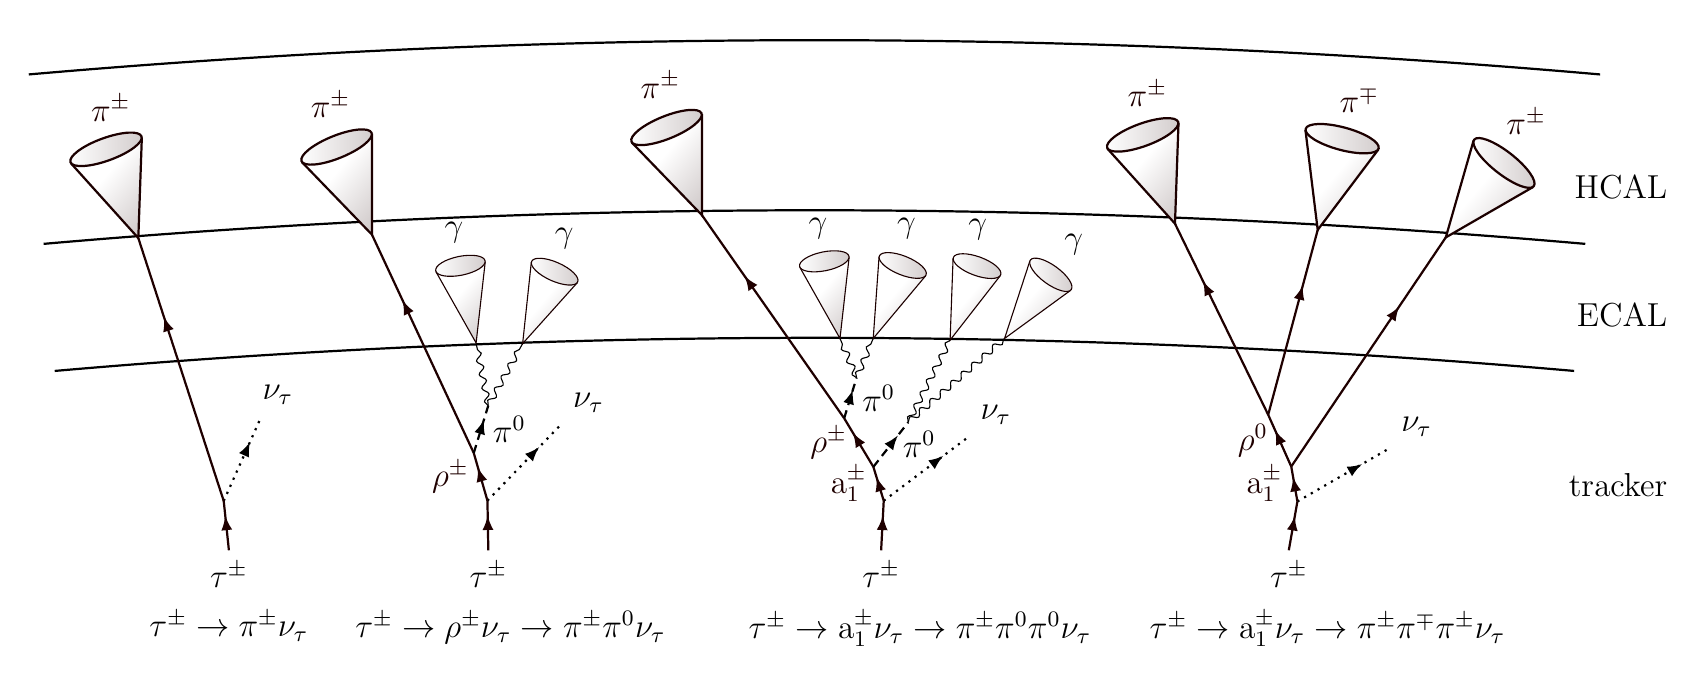
\begin{tikzpicture}[scale=0.9]
  \large
  \def\R{120}            % inner radius
  \def\hca{5}            % half central angle
  \def\hcl{\R*sin(\hca)} % half chord length c = 2Rsin(theta/2)
  \def\tracker{3}        % tracker
  \def\ECAL{4.8}         % ECAL
  \def\HCAL{7.2}         % HCAL
  
  % SUBDETECTORS
  \subdetectors
  
  % DM 0
  \begin{scope}[shift={({-0.79*\hcl},0)},rotate=6]
    \node[below] at (0,0) {$\tau^\pm$};
    \node[below=18] at (0,0) {$\tau^\pm\to\pi^\pm\nu_\tau$};
    \draw[charged] % tau
      (0,0) -- (0,0.7) coordinate (tau);
    \draw[neutrino,rotate=-30] % neutrinos
      (tau) --+ (0,1.3) node[right=6pt,above] {$\nu_\tau$};
    \draw[charged,rotate=12] % pion
      (tau) --+ (0,3.9) node[left=10,above=38] {$\pi^\pm$}
      pic[rotate=20,scale=1.2] {cone};
  \end{scope}
  
  % DM 1
  \begin{scope}[shift={({-0.44*\hcl},0)},rotate=1]
    \node[below] at (0,0) {$\tau^\pm$};
    \node[right=8pt,below=18] at (0,0) {$\tau^\pm\to\rho^\pm\nu_\tau\to\pi^\pm\pi^0\nu_\tau$};
    \draw[charged] % tau
      (0,0) -- (0,0.7) coordinate (tau);
    \draw[neutrino,rotate=-45] % neutrinos
      (tau) --+ (0,1.5) node[above right] {$\nu_\tau$};
    \draw[charged,rotate=15] % rho
      (tau) --+ (0,0.7) coordinate (rho) node[midway,left] {$\rho^\pm$};
    \draw[charged,rotate=24] % pion
      (rho) --+ (0,3.4) node[left=15,above=38] {$\pi^\pm$}
      pic[rotate=22,scale=1.2] {cone};
    \draw[neutral,rotate=-18] % pion0
      (rho) --+ (0,0.7) coordinate (pion0) node[midway,right] {$\pi^0$};
    \draw[photon,rotate=10] % photon 1
      (pion0) --+ (0,0.9) node[left=8,above=32] {$\gamma$}
      pic[rotate=11.5,xscale=0.8] {cone};
    \draw[photon,rotate=-30] % photon 2
      (pion0) --+ (0,1.0) node[right=15,above=30] {$\gamma$}
      pic[rotate=-24,xscale=0.8] {cone};
  \end{scope}
  
  % DM 2
  \begin{scope}[shift={({0.09*\hcl},0)},rotate=-3]
    \node[below] (0,0) {$\tau^\pm$};
    \node[right=14pt,below=18] at (0,0) {$\tau^\pm\to\text{a}_1^\pm\nu_\tau\to\pi^\pm\pi^0\pi^0\nu_\tau$};
    \draw[charged] % tau
      (0,0) -- (0,0.7) coordinate (tau);
    \draw[neutrino,rotate=-50] % neutrinos
      (tau) --+ (0,1.5) node[above right] {$\nu_\tau$};
    \draw[charged,rotate=20] % a1
      (tau) --+ (0,0.5) coordinate (a1) node[midway,left] {$\text{a}_1^\pm$};
    \draw[charged,rotate=34] % rho
      (a1) --+ (0,0.8) coordinate (rho) node[midway,left] {$\rho^\pm$};
    \draw[charged,rotate=38] % pion
      (rho) --+ (0,3.5) node[left=15,above=38] {$\pi^\pm$}
      pic[rotate=22,scale=1.2] {cone};
    \draw[neutral,rotate=-35] % pion0
      (a1) --+ (0,0.8) coordinate (pion01) node[midway,right] {$\pi^0$};
    \draw[neutral,rotate=-14] % pion0
      (rho) --+ (0,0.6) coordinate (pion02) node[midway,right] {$\pi^0$};
    \draw[photon,rotate=26] % photon 1
      (pion02) --+ (0,0.6) node[left=8,above=32] {$\gamma$}
      pic[rotate=11.5,xscale=0.8] {cone};
    \draw[photon,rotate=-20] % photon 2
      (pion02) --+ (0,0.6) node[right=12,above=32] {$\gamma$}
      pic[rotate=-22,xscale=0.8] {cone};
    \draw[photon,rotate=-24] % photon 3
      (pion01) --+ (0,1.3) node[right=10,above=32] {$\gamma$}
      pic[rotate=-20,xscale=0.8] {cone};
    \draw[photon,rotate=-46] % photon 4
      (pion01) --+ (0,1.8) node[right=25,above=26] {$\gamma$}
      pic[rotate=-36,xscale=0.8] {cone};
  \end{scope}
  
  % DM 10
  \begin{scope}[shift={({0.64*\hcl},0)},rotate=-10]
    \node[below] (0,0) {$\tau^\pm$};
    \node[right=14pt,below=18] at (0,0) {$\tau^\pm\to\text{a}_1^\pm\nu_\tau\to\pi^\pm\pi^\mp\pi^\pm\nu_\tau$};
    \draw[charged] % tau
      (0,0) -- (0,0.7) coordinate (tau);
    \draw[neutrino,rotate=-50] % neutrinos
      (tau) --+ (0,1.5) node[above right] {$\nu_\tau$};
    \draw[charged,rotate=20] % a1
      (tau) --+ (0,0.5) coordinate (a1) node[midway,left] {$\text{a}_1^\pm$};
    \draw[charged,rotate=34] % rho
      (a1) --+ (0,0.8) coordinate (rho) node[midway,left] {$\rho^0$};
    \draw[charged,rotate=36] % pion 1
      (rho) --+ (0,3.0) node[left=10,above=38] {$\pi^\pm$}
      pic[rotate=20,scale=1.2] {cone};
    \draw[charged,rotate=-5] % pion 2
      (rho) --+ (0,2.7) node[right=15,above=38] {$\pi^\mp$}
      pic[rotate=-15,scale=1.2] {cone};
    \draw[charged,rotate=-24] % pion 3
      (a1) --+ (0,3.9) node[right=29,above=33] {$\pi^\pm$}
      pic[rotate=-38,scale=1.2] {cone};
  \end{scope}
  
\end{tikzpicture}


% TAU DECAY MODES 0, 1, 10
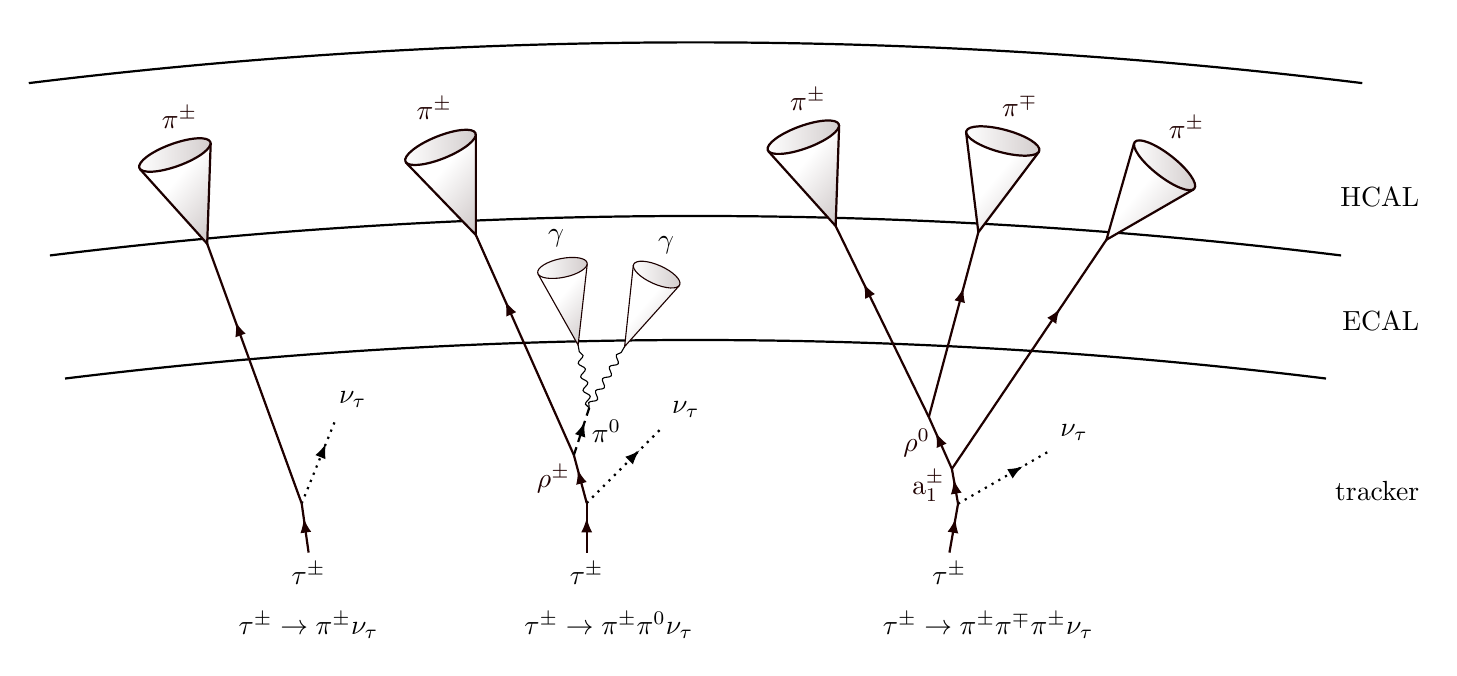
\begin{tikzpicture}[scale=0.9]
  \def\R{70}             % inner radius
  \def\hca{7}            % half central angle
  \def\hcl{\R*sin(\hca)} % half chord length c = 2Rsin(theta/2)
  \def\tracker{3}        % tracker
  \def\ECAL{4.75}        % ECAL
  \def\HCAL{7.2}         % HCAL
  
  % SUBDETECTORS
  \subdetectors
  
  % DM 0
  \begin{scope}[shift={({-0.64*\hcl},0)},rotate=8]
    \node[below] at (0,0) {$\tau^\pm$};
    \node[below=18] at (0,0) {$\tau^\pm\to\pi^\pm\nu_\tau$};
    \draw[charged]                   % tau
      (0,0) -- (0,0.7) coordinate (tau);
    \draw[neutrino,rotate=-30] % neutrinos
      (tau) --+ (0,1.3) node[right=6pt,above] {$\nu_\tau$};
    \draw[charged,rotate=12] % pion
      (tau) --+ (0,3.9) node[left=10,above=38] {$\pi^\pm$}
      pic[rotate=20,scale=1.2] {cone};
  \end{scope}
  
  % DM 1
  \begin{scope}[shift={({-0.18*\hcl},0)},rotate=0]
    \node[below] at (0,0) {$\tau^\pm$};
    \node[right=8pt,below=18] at (0,0) {$\tau^\pm\to\pi^\pm\pi^0\nu_\tau$};
    \draw[charged]                   % tau
      (0,0) -- (0,0.7) coordinate (tau);
    \draw[neutrino,rotate=-45] % neutrinos
      (tau) --+ (0,1.5) node[above right] {$\nu_\tau$};
    \draw[charged,rotate=15] % rho
      (tau) --+ (0,0.7) coordinate (rho) node[midway,left] {$\rho^\pm$};
    \draw[charged,rotate=24] % pion
      (rho) --+ (0,3.4) node[left=15,above=38] {$\pi^\pm$}
      pic[rotate=22,scale=1.2] {cone};
    \draw[neutral,rotate=-18] % pion0
      (rho) --+ (0,0.7) coordinate (pion0) node[midway,right] {$\pi^0$};
    \draw[photon,rotate=10] % photon 1
      (pion0) --+ (0,0.9) node[left=8,above=32] {$\gamma$}
      pic[rotate=11.5,xscale=0.8] {cone};
    \draw[photon,rotate=-30] % photon 2
      (pion0) --+ (0,1.0) node[right=15,above=30] {$\gamma$}
      pic[rotate=-24,xscale=0.8] {cone};
  \end{scope}
  
  % DM 10
  \begin{scope}[shift={({0.42*\hcl},0)},rotate=-10]
    \node[below] (0,0) {$\tau^\pm$};
    \node[right=14pt,below=18] at (0,0) {$\tau^\pm\to\pi^\pm\pi^\mp\pi^\pm\nu_\tau$};
    \draw[charged] % tau
      (0,0) -- (0,0.7) coordinate (tau);
    \draw[neutrino,rotate=-50] % neutrinos
      (tau) --+ (0,1.5) node[above right] {$\nu_\tau$};
    \draw[charged,rotate=20] % a1
      (tau) --+ (0,0.5) coordinate (a1) node[midway,left] {$\text{a}_1^\pm$};
    \draw[charged,rotate=34] % rho
      (a1) --+ (0,0.8) coordinate (rho) node[midway,left] {$\rho^0$};
    \draw[charged,rotate=36] % pion 1
      (rho) --+ (0,3.0) node[left=10,above=38] {$\pi^\pm$}
      pic[rotate=20,scale=1.2] {cone};
    \draw[charged,rotate=-5] % pion 2
      (rho) --+ (0,2.7) node[right=15,above=38] {$\pi^\mp$}
      pic[rotate=-15,scale=1.2] {cone};
    \draw[charged,rotate=-24] % pion 3
      (a1) --+ (0,3.9) node[right=29,above=33] {$\pi^\pm$}
      pic[rotate=-38,scale=1.2] {cone};
  \end{scope}
  
\end{tikzpicture}


% TAU DECAY MODE 1 only
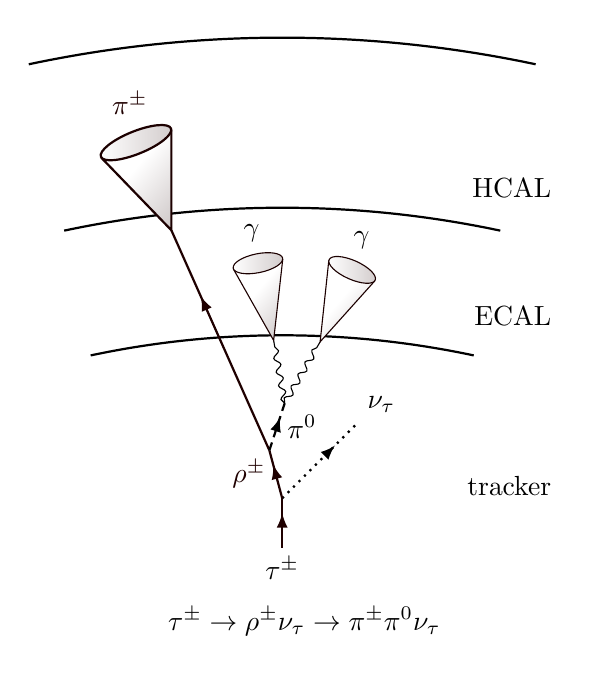
\begin{tikzpicture}[scale=0.9]
  \def\R{10}             % inner radius
  \def\hca{12}           % half central angle
  \def\hcl{\R*sin(\hca)} % half chord length c = 2Rsin(theta/2)
  \def\tracker{3}        % tracker
  \def\ECAL{4.8}         % ECAL
  \def\HCAL{7.2}         % HCAL
  
  % SUBDETECTORS
  \subdetectors
  
  % DM 1
  \begin{scope}[shift={(0,0)},rotate=0]
    \node[below] at (0,0) {$\tau^\pm$};
    \node[right=8pt,below=18] at (0,0) {$\tau^\pm\to\rho^\pm\nu_\tau\to\pi^\pm\pi^0\nu_\tau$};
    \draw[charged] % tau
      (0,0) -- (0,0.7) coordinate (tau);
    \draw[neutrino] % neutrinos
      (tau) --+ (45:1.5) node[above right] {$\nu_\tau$};
    \draw[charged] % rho
      (tau) --+ (105:0.7) coordinate (rho) node[midway,left] {$\rho^\pm$};
    \draw[charged] % pion
      (rho) --+ (114:3.4) node[left=15,above=38] {$\pi^\pm$}
      pic[rotate=22,scale=1.2] {cone};
    \draw[neutral] % pion0
      (rho) --+ (72:0.7) coordinate (pion0) node[midway,right] {$\pi^0$};
    \draw[photon] % photon 1
      (pion0) --+ (100:0.9) node[left=8,above=32] {$\gamma$}
      pic[rotate=11.5,xscale=0.8] {cone};
    \draw[photon] % photon 2
      (pion0) --+ (60:1.0) node[right=15,above=30] {$\gamma$}
      pic[rotate=-24,xscale=0.8] {cone};
  \end{scope}
  
\end{tikzpicture}


% TAU DECAY MODE 1 only - colored
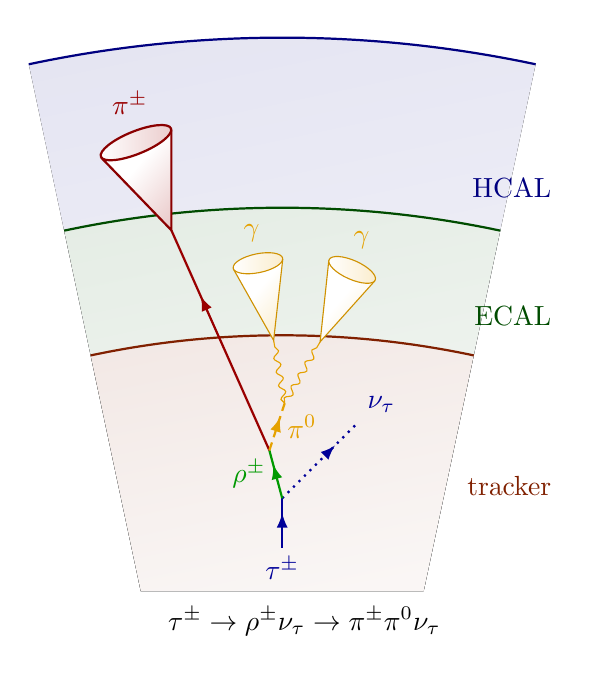
\begin{tikzpicture}[scale=0.9]
  \def\R{10}             % inner radius
  \def\hca{12}           % half central angle
  \def\hcl{\R*sin(\hca)} % half chord length c = 2Rsin(theta/2)
  \def\tracker{3}        % tracker
  \def\ECAL{4.8}         % ECAL
  \def\HCAL{7.2}         % HCAL
  
  % SUBDETECTORS
  \subdetectorscol
  
  % DM 1
  \begin{scope}[shift={(0,0)},rotate=0]
    \node[below,taucol] at (0,0) {$\tau^\pm$};
    \node[right=8pt,below=18] at (0,0) {$\tau^\pm\to\rho^\pm\nu_\tau\to\pi^\pm\pi^0\nu_\tau$};
    \draw[charged,taucol] % tau
      (0,0) -- (0,0.7) coordinate (tau);
    \draw[neutrino,taucol] % neutrinos
      (tau) --+ (45:1.5) node[above right] {$\nu_\tau$};
    \draw[charged,rhocol] % rho
      (tau) --+ (105:0.7) coordinate (rho) node[midway,left] {$\rho^\pm$};
    \draw[charged,hadroncol] % pion
      (rho) --++ (114:3.4) node[left=15,above=38] {$\pi^\pm$}
      pic[rotate=22,scale=1.2] {cone=hadroncol};
    \draw[neutral,photoncol] % pion0
      (rho) --+ (72:0.7) coordinate (pion0) node[midway,right] {$\pi^0$};
    \draw[photon,photoncol] % photon 1
      (pion0) --+ (100:0.9) node[left=8,above=32] {$\gamma$}
      pic[rotate=11.5,xscale=0.8] {cone=photoncol};
    \draw[photon,photoncol] % photon 2
      (pion0) --+ (60:1.0) node[right=15,above=30] {$\gamma$}
      pic[rotate=-24,xscale=0.8] {cone=photoncol};
  \end{scope}
  
\end{tikzpicture}


% TAU DECAY MODE 10 only
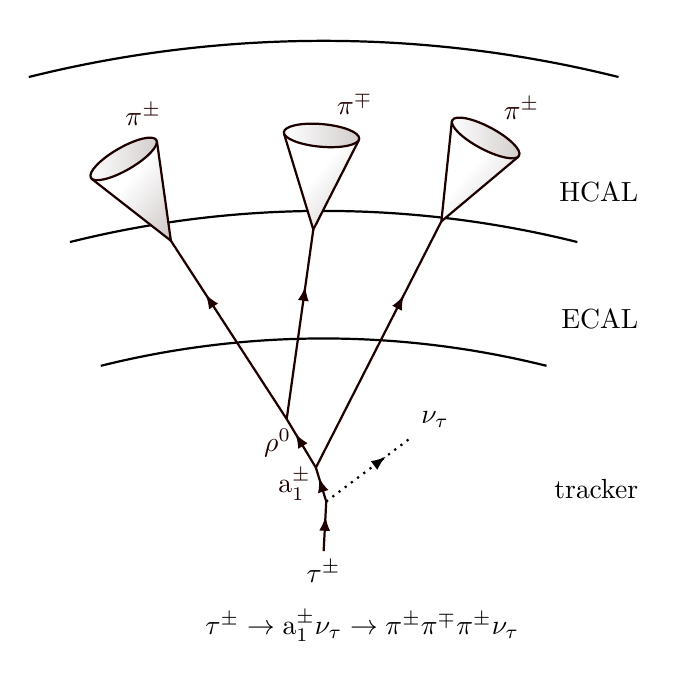
\begin{tikzpicture}[scale=0.9]
  \def\R{10}             % inner radius
  \def\hca{14}           % half central angle
  \def\hcl{\R*sin(\hca)} % half chord length c = 2Rsin(theta/2)
  \def\tracker{3}        % tracker
  \def\ECAL{4.8}         % ECAL
  \def\HCAL{7.2}         % HCAL
  
  % SUBDETECTORS
  \subdetectors
  
  % DM 10
  \begin{scope}[shift={(0,0)},rotate=-3]
    \node[below] (0,0) {$\tau^\pm$};
    \node[right=14pt,below=18] at (0,0) {$\tau^\pm\to\text{a}_1^\pm\nu_\tau\to\pi^\pm\pi^\mp\pi^\pm\nu_\tau$};
    \draw[charged] % tau
      (0,0) -- (0,0.7) coordinate (tau);
    \draw[neutrino] % neutrinos
      (tau) --+ (40:1.5) node[above right] {$\nu_\tau$};
    \draw[charged] % a1
      (tau) --+ (110:0.5) coordinate (a1) node[midway,left] {$\text{a}_1^\pm$};
    \draw[charged] % rho
      (a1) --+ (124:0.8) coordinate (rho) node[midway,left] {$\rho^0$};
    \draw[charged,rotate=36] % pion 1
      (rho) --+ (0,3.0) node[left=10,above=38] {$\pi^\pm$}
      pic[rotate=30,scale=1.2] {cone};
    \draw[charged] % pion 2
      (rho) --+ (85:2.7) node[right=15,above=38] {$\pi^\mp$}
      pic[rotate=-5,scale=1.2] {cone};
    \draw[charged] % pion 3
      (a1) --+ (66:3.9) node[right=29,above=33] {$\pi^\pm$}
      pic[rotate=-28,scale=1.2] {cone};
  \end{scope}
  
\end{tikzpicture}


\end{document}